\section{Physikalische Grundlagen}
\subsection{Radioaktiver Zerfall und Strahlung}

Der \textalpha- und \textbeta-Zerfall der verwendeten Proben führt dazu,
dass sich nach dem Zerfall die Kerne in angeregten Zuständen befinden.
Diese Anregungsenergie wird dann als \textgamma-Photon abgegeben.\\[\baselineskip]
Der \textalpha-Zerfall, der fünf mal in der Zerfallsreihe von ${}^{228}$Th auftritt,
findet nach folgendem Schema statt:
\begin{center}
${}^{A}_{Z}\text{X} \rightarrow {}^{A-4}_{Z-2}\text{Y} + {}^{4}_{2}\text{He}$
\end{center}
Der Mutterkern X mit Protonenzahl Z und Nukleonenzahl A zerfällt unter Aussendung eines Helium-Kerns
in den Tochterkern Y.\\[\baselineskip]
Beim \textbeta$^-$-Zerfall zerfällt ein Neutron im Kern zu einem Proton, einem Elektron und einem
Antielektronenneutrino:
\begin{center}
$\text{n} \rightarrow \text{p}^+ + \text{e}^- +\bar{\nu_{\text{e}}}$ bzw.\\[0.15cm]
${}^{A}_{Z}\text{X} \rightarrow {}^{A}_{Z+1}\text{Y} + \text{e}^- + \bar{\nu_{\text{e}}}$
\end{center}

Der \textbeta$^-$-Zerfall tritt zwei mal in der Zerfallsreihe von ${}^{228}$Th auf.
Auch ${}^{60}$Co und ${}^{152}$Eu sind \textbeta$^-$-Strahler.

${}^{22}$Na ist ein \textbeta$^+$-Strahler:
Hier zerfällt ein Proton im Kern zu einem Neutron, einem Positron und einem
Elektronenneutrino:
\begin{center}
$\text{p}^+ \rightarrow \text{n} + \text{e}^+ +\nu_{\text{e}}$ bzw.\\[0.15cm]
${}^{A}_{Z}\text{X} \rightarrow {}^{A}_{Z-1}\text{Y} + \text{e}^+ + \nu_{\text{e}}$
\end{center}

Das Positron kann in Materie für nur sehr kurze Zeit existieren und zerstrahlt mit einem Elektron
in zwei Photonen mit je 511\,keV Energie, die in einem Winkel von 180$^\circ$ emittiert werden.

Die emittierten \textgamma-Photonen können auf verschiedene Arten mit Materie wechselwirken:
Beim \emph{Photoeffekt} absorbieren gebundene Elektronen das Photon und verlassen mit hoher Geschwindigkeit das Atom.
Beim \emph{Comptoneffekt} findet elastische Streuung von Photonen an freien Elektronen statt.
Ein Teil der Photonenenergie wird so auf das Elektron übertragen.
Eine weitere Möglichkeit ist die \emph{Paarbildung}, bei der im Feld eines Atomkerns aus einem energiereichen
Photon ein Elektron-Positron-Paar entsteht.



\subsection{Szintillatoren}
Die Wechselwirkung von Strahlung mit Materie wird in Szintillationszählern zur Energiemessung genutzt:
Durch die Strahlung werden Elektronen im Szintillatormaterial angeregt.
Die Anregungsenergie beträgt dabei wenige Elektronenvolt und die Zahl der angeregten Elektronen
ist (im Idealfall, bei vollständiger Absorption) proportional zur Energie der Strahlung.
Um das sichtbare Licht, das emittiert wird, wenn die Elektronen in den Grundzustand zurückfallen,
messen zu können, muss das Szintillatormaterial für das Licht dieser Wellenlänge transparent sein.\\
Dies wird im NaI-Kristall durch eine Dotierung mit Thallium erreicht.
Die Störstellen, die dadurch im Gitter entstehen,
erzeugen neue Energieniveaus zwischen Valenzband und Leitungsband und wirken als
Rekombinationszentren, an denen ein Übergang angeregter Elektronen in den Grundzustand erfolgen kann.
Ein Photon, das dabei emittiert wird, wird nur zu einer sehr geringen Wahrscheinlichkeit
wieder absorbiert.\\
Die Lebensdauer der angeregten Zustände bestimmt dabei die Zeitauflösung des Szintillators:
Bei dem anorganischen NaI-Kristall liegt sie im \textmu s-Bereich und ist damit deutlich
höher als bei organischen Szintillatoren.
Bei der Lichtausbeute und damit der möglichen Energieauflösung ist sind anorganische
Szintillatoren allerdings besser.\\
Bei dem Plastik-Szintillator wird die Transparenz durch Zugabe von Anthracen als Aktivatorsubstanz erreicht.
Einfallende Strahlung regt Moleküle des Plasikmaterials an und diese Anregungsenergie wird auf die Anthracenmoleküle
übertragen. Beim Übergang der Moleküle in den Grundzustand wird Strahlung emittiert,
für die das Material transparent ist.\\
Die Strahlung, die aus dem Szintillationszähler austritt,
gelangt dann in einen Photomultiplier und wird dort in einen Strom proportional zur Intensität umgewandelt.

\subsection{Photomultiplier}

\begin{figure}[H]
\begin{center}
  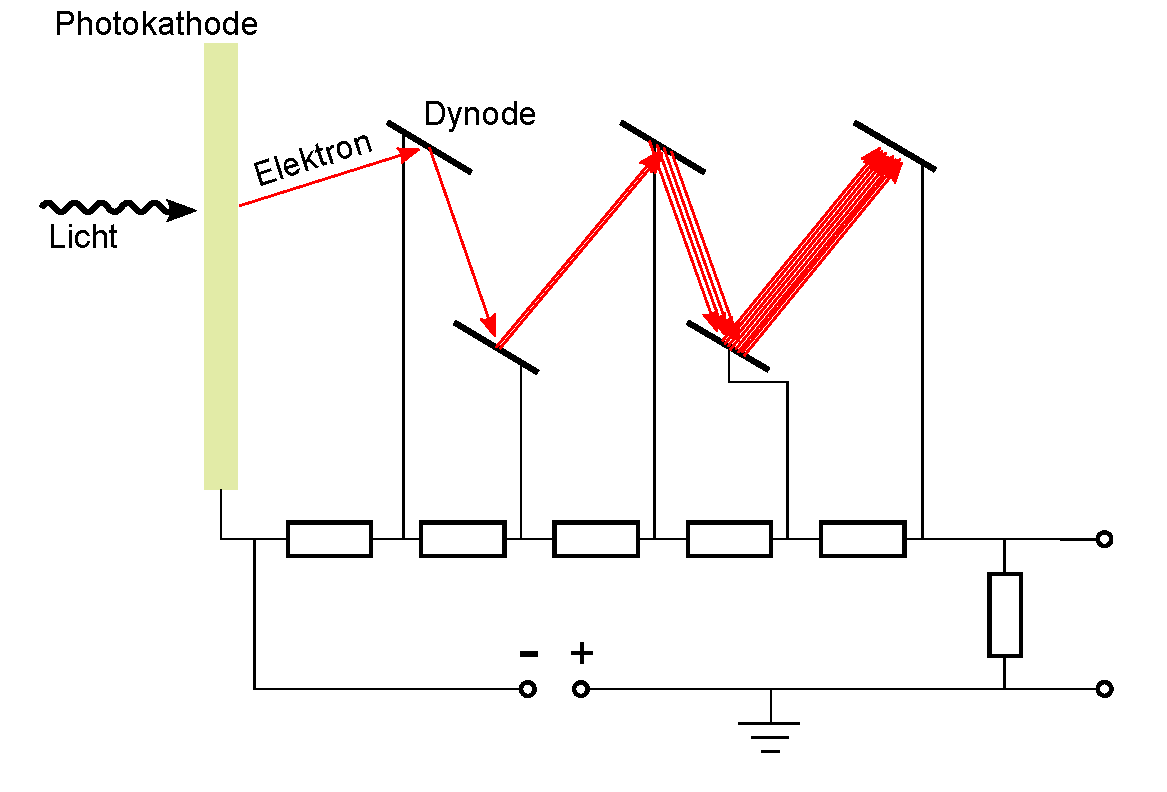
\includegraphics[width=\textwidth]{../img/photomultiplier.pdf}
  \caption[---]{Aufbau eines Photomultipliers zur Umwandlung von schwachen Lichtsignalen in Strompulse.}
  \label{img:aufbau}
\end{center}
\end{figure}